% Reusable TikZ diagrams for the AIΩN Foundations Series
% Requires: \usepackage{tikz} with libraries positioning,calc

% Diagram A — WARP skeleton with attachments
\newcommand{\DiagramWARPSkeleton}{
  \begin{tikzpicture}[>=stealth, node distance=2cm]
    \node[circle, draw, thick] (v1) {$v_1$};
    \node[circle, draw, thick, right of=v1] (v2) {$v_2$};
    \draw[->, thick] (v1) -- node[above] {$e$} (v2);
    \node[rectangle, draw, dashed, below=8pt of v1] (a1) {\small WARP};
    \draw[dashed] (v1) -- (a1);
    \node[rectangle, draw, dashed, below=8pt of v2] (a2) {\small WARP};
    \draw[dashed] (v2) -- (a2);
    \node[rectangle, draw, dashed, below=8pt of $(v1)!0.5!(v2)$] (ae) {\small WARP};
    \draw[dashed] ($(v1)!0.5!(v2)$) -- (ae);
  \end{tikzpicture}}

\newcommand{\AttachmentSep}{80pt}
\newcommand{\EdgeAttachmentSep}{68pt}

% Diagram A2 — Working example with payload labels
\newcommand{\DiagramCallGraphExample}{
  \begin{tikzpicture}[>=stealth, node distance=5.2cm, every node/.style={font=\small}]
    % Skeleton
    \node[circle, draw, very thick, inner sep=3pt] (vf) {$v_f$};
    \node[circle, draw, very thick, inner sep=3pt, right of=vf] (vg) {$v_g$};
    \draw[->, very thick] (vf) -- node[above=10pt] {$e_{\mathrm{call}}$} (vg);
    % Attachments
    \node[rectangle, draw, very thick, rounded corners=4pt, fill=blue!12, inner sep=5pt, below=\AttachmentSep of vf, xshift=-8pt] (astf) {AST($f$)};
    \node[rectangle, draw, very thick, rounded corners=4pt, fill=blue!12, inner sep=5pt, below=\AttachmentSep of vg, xshift=8pt] (astg) {AST($g$)};
    \node[rectangle, draw, very thick, rounded corners=6pt, fill=green!18, inner sep=6pt, below=\EdgeAttachmentSep of $(vf)!0.5!(vg)$] (prov) {Provenance / profiling};
    \draw[dashed, very thick] (vf.south) -- ++(0,-10pt) |- (astf.north);
    \draw[dashed, very thick] (vg.south) -- ++(0,-10pt) |- (astg.north);
    \draw[dashed, very thick] ($(vf)!0.5!(vg)$) -- ++(0,-10pt) |- (prov.north);
    % Nested WARPs inside attachments (to show recursion)
    \node[rectangle, draw, dashed, inner sep=3pt, below=16pt of astf] (astfsub) {\tiny $\bullet\!\!\!\to\!\!\!\bullet$};
    \draw[dashed, thick] (astf.south) -- (astfsub.north);
    \node[rectangle, draw, dashed, inner sep=3pt, below=16pt of astg] (astgsub) {\tiny $\bullet\!\!\!\leftarrow\!\!\!\bullet$};
    \draw[dashed, thick] (astg.south) -- (astgsub.north);
    \node[rectangle, draw, dashed, inner sep=3pt, below=16pt of prov] (provsub) {\tiny $\bullet\!-\!\bullet\!-\!\bullet$};
    \draw[dashed, thick] (prov.south) -- (provsub.north);
  \end{tikzpicture}}

\definecolor{LevelZeroAtom}{RGB}{90,90,90}
\definecolor{LevelZeroEdge}{RGB}{60,60,60}
\definecolor{LevelOneNode}{RGB}{160,200,255}
\definecolor{LevelOneEdge}{RGB}{40,110,200}
\definecolor{LevelTwoNode}{RGB}{255,182,193}
\definecolor{LevelTwoEdge}{RGB}{200,60,60}

% Diagram A1b — Tiny WARP: 3 vertices, 2 edges, atom attachments
\newcommand{\DiagramNestedWARP}{
  \begin{tikzpicture}[>=stealth, every node/.style={font=\small}]
    % Styles
    \tikzset{
      lvl2/.style={circle, draw=LevelTwoEdge, fill=LevelTwoNode!85, line width=1.8pt, minimum size=12mm},
      lvl2edge/.style={draw=LevelTwoEdge, line width=1.8pt},
      lvl1/.style={circle, draw=LevelOneEdge, fill=LevelOneNode!85, line width=1.5pt, minimum size=11mm},
      lvl1edge/.style={draw=LevelOneEdge, line width=1.5pt},
      atom/.style={circle, draw=LevelZeroEdge, fill=LevelZeroAtom!45, minimum size=5.5pt, inner sep=1pt},
      attachline/.style={dashed, thick, draw=black!70},
      note/.style={font=\scriptsize}
    }

    % Skeleton vertices (level 2)
    \node[lvl2,label=above:{\scriptsize $w_1$}] (w1) {};
    \node[lvl2,label=above:{\scriptsize $w_2$}, right=3.2cm of w1] (w2) {};
    \node[lvl2,label=above:{\scriptsize $w_3$}, right=3.2cm of w2] (w3) {};

    % Edges (level 2)
    \draw[lvl2edge,->] (w1) -- node[above, note] {$e_1$} (w2);
    \draw[lvl2edge,->] (w2) -- node[above, note] {$e_2$} (w3);

    % Atom attachments on w1, w3
    \node[atom, below=1.1cm of w1] (a1) {};
    \node[atom, below=1.1cm of w3] (a3) {};
    \draw[attachline] (w1) -- (a1);
    \draw[attachline] (w3) -- (a3);

    % Atom attachments on edges e1, e2
    \node[atom, below=1.0cm of $(w1)!0.5!(w2)$] (ae1) {};
    \node[atom, below=1.0cm of $(w2)!0.5!(w3)$] (ae2) {};
    \draw[attachline] ($(w1)!0.5!(w2)$) -- (ae1);
    \draw[attachline] ($(w2)!0.5!(w3)$) -- (ae2);

    % Nested WARP on w2 (level 1, blue)
    \node[lvl1, below=1.4cm of w2, label=above:{\scriptsize $u$}] (u) {};
    \node[lvl1, right=2.6cm of u, label=above:{\scriptsize $v$}] (v) {};
    \draw[lvl1edge,->] (u) -- node[above, note] {$e$} (v);

    % Atom attachments for the nested WARP
    \node[atom, below=1.0cm of u] (au) {};
    \node[atom, below=1.0cm of v] (av) {};
    \node[atom, below=1.0cm of $(u)!0.5!(v)$] (ae) {};
    \draw[attachline] (u) -- (au);
    \draw[attachline] (v) -- (av);
    \draw[attachline] ($(u)!0.5!(v)$) -- (ae);

    % Arrow showing w2 attaches the inner WARP
    \draw[attachline,->,>=stealth, ultra thick] (w2.south) -- ++(0,-0.3) |- (u.north);

    % Legend text
    \node[note, below=0.35cm of ae] {atoms};
    \node[note, above=0.25cm of u] {inner WARP $X_1$};
    \node[note, above=0.35cm of w2] {outer skeleton $X_2$};
  \end{tikzpicture}}

% Diagram A3 — Compiler pipeline snapshot
\newcommand{\DiagramCompilerPipeline}{
  \begin{tikzpicture}[>=stealth, node distance=2.6cm, every node/.style={font=\small}]
    % stages
    \node[rectangle, draw, very thick, rounded corners=3pt, fill=blue!8, inner sep=5pt] (p) {parse};
    \node[rectangle, draw, very thick, rounded corners=3pt, fill=blue!8, inner sep=5pt, right=2.6cm of p] (t) {typecheck};
    \node[rectangle, draw, very thick, rounded corners=3pt, fill=blue!8, inner sep=5pt, right=2.6cm of t] (o) {opt};
    \node[rectangle, draw, very thick, rounded corners=3pt, fill=blue!8, inner sep=5pt, right=2.6cm of o] (c) {codegen};
    \draw[->, very thick] (p) -- (t);
    \draw[->, very thick] (t) -- (o);
    \draw[->, very thick] (o) -- (c);
    % attachments under each stage
    \node[rectangle, draw, rounded corners=3pt, fill=green!18, inner sep=4pt, below=24pt of p] (patt) {AST};
    \node[rectangle, draw, rounded corners=3pt, fill=green!18, inner sep=4pt, below=24pt of t] (tatt) {typed core};
    \node[rectangle, draw, rounded corners=3pt, fill=green!18, inner sep=4pt, below=24pt of o] (oatt) {SSA CFG};
    \node[rectangle, draw, rounded corners=3pt, fill=green!18, inner sep=4pt, below=24pt of c] (catt) {target DAG};
    \draw[dashed, very thick] (p.south) -- (patt.north);
    \draw[dashed, very thick] (t.south) -- (tatt.north);
    \draw[dashed, very thick] (o.south) -- (oatt.north);
    \draw[dashed, very thick] (c.south) -- (catt.north);
    % edge provenance
    \node[rectangle, draw, rounded corners=3pt, fill=orange!20, inner sep=4pt, below=28pt of $(p)!0.5!(t)$] (prov1) {rewrite log};
    \node[rectangle, draw, rounded corners=3pt, fill=orange!20, inner sep=4pt, below=28pt of $(t)!0.5!(o)$] (prov2) {passes + timings};
    \node[rectangle, draw, rounded corners=3pt, fill=orange!20, inner sep=4pt, below=28pt of $(o)!0.5!(c)$] (prov3) {backend opts};
    \draw[dashed, very thick] ($(p)!0.5!(t)$) -- (prov1.north);
    \draw[dashed, very thick] ($(t)!0.5!(o)$) -- (prov2.north);
    \draw[dashed, very thick] ($(o)!0.5!(c)$) -- (prov3.north);
  \end{tikzpicture}}

% Diagram A4 — Microservice call with lineage
\newcommand{\DiagramMicroservice}{
  \begin{tikzpicture}[>=stealth, node distance=2.9cm, every node/.style={font=\small}]
    \node[rectangle, draw, very thick, rounded corners=3pt, fill=blue!8, inner sep=5pt] (fe) {frontend};
    \node[rectangle, draw, very thick, rounded corners=3pt, fill=blue!8, inner sep=5pt, right=2.9cm of fe] (au) {auth};
    \node[rectangle, draw, very thick, rounded corners=3pt, fill=blue!8, inner sep=5pt, right=2.9cm of au] (or) {orders};
    \node[rectangle, draw, very thick, rounded corners=3pt, fill=blue!8, inner sep=5pt, right=2.9cm of or] (bi) {billing};
    \draw[->, very thick] (fe) -- (au);
    \draw[->, very thick] (au) -- (or);
    \draw[->, very thick] (or) -- (bi);
    % attachments (local dataflow)
    \node[rectangle, draw, rounded corners=3pt, fill=green!18, inner sep=4pt, below=24pt of fe] (featt) {UI dataflow};
    \node[rectangle, draw, rounded corners=3pt, fill=green!18, inner sep=4pt, below=24pt of au] (auatt) {token check DAG};
    \node[rectangle, draw, rounded corners=3pt, fill=green!18, inner sep=4pt, below=24pt of or] (oratt) {order enrichment};
    \node[rectangle, draw, rounded corners=3pt, fill=green!18, inner sep=4pt, below=24pt of bi] (biatt) {charge calc};
    \draw[dashed, very thick] (fe.south) -- (featt.north);
    \draw[dashed, very thick] (au.south) -- (auatt.north);
    \draw[dashed, very thick] (or.south) -- (oratt.north);
    \draw[dashed, very thick] (bi.south) -- (biatt.north);
    % edge lineage
    \node[rectangle, draw, rounded corners=3pt, fill=orange!20, inner sep=4pt, below=28pt of $(fe)!0.5!(au)$] (l1) {trace ID + headers};
    \node[rectangle, draw, rounded corners=3pt, fill=orange!20, inner sep=4pt, below=28pt of $(au)!0.5!(or)$] (l2) {retries / spans};
    \node[rectangle, draw, rounded corners=3pt, fill=orange!20, inner sep=4pt, below=28pt of $(or)!0.5!(bi)$] (l3) {audit + latency};
    \draw[dashed, very thick] ($(fe)!0.5!(au)$) -- (l1.north);
    \draw[dashed, very thick] ($(au)!0.5!(or)$) -- (l2.north);
    \draw[dashed, very thick] ($(or)!0.5!(bi)$) -- (l3.north);
  \end{tikzpicture}}

% Diagram A5 — Robotics task plan
\newcommand{\DiagramRobotics}{
  \begin{tikzpicture}[>=stealth, node distance=3.2cm, every node/.style={font=\small}]
    \node[rectangle, draw, very thick, rounded corners=3pt, fill=blue!8, inner sep=5pt] (per) {perceive};
    \node[rectangle, draw, very thick, rounded corners=3pt, fill=blue!8, inner sep=5pt, right=3.2cm of per] (pla) {plan};
    \node[rectangle, draw, very thick, rounded corners=3pt, fill=blue!8, inner sep=5pt, right=3.2cm of pla] (act) {act};
    \draw[->, very thick] (per) -- (pla);
    \draw[->, very thick] (pla) -- (act);
    % attachments
    \node[rectangle, draw, rounded corners=3pt, fill=green!18, inner sep=4pt, below=28pt of per] (peratt) {sensor fusion DAG};
    \node[rectangle, draw, rounded corners=3pt, fill=green!18, inner sep=4pt, below=28pt of pla] (platt) {search tree};
    \node[rectangle, draw, rounded corners=3pt, fill=green!18, inner sep=4pt, below=28pt of act] (actatt) {motor seq + timing};
    \draw[dashed, very thick] (per.south) -- (peratt.north);
    \draw[dashed, very thick] (pla.south) -- (platt.north);
    \draw[dashed, very thick] (act.south) -- (actatt.north);
    % edge safety evidence
    \node[rectangle, draw, rounded corners=3pt, fill=orange!20, inner sep=4pt, below=32pt of $(per)!0.5!(pla)$] (s1) {perception certs};
    \node[rectangle, draw, rounded corners=3pt, fill=orange!20, inner sep=4pt, below=32pt of $(pla)!0.5!(act)$] (s2) {collision checks};
    \draw[dashed, very thick] ($(per)!0.5!(pla)$) -- (s1.north);
    \draw[dashed, very thick] ($(pla)!0.5!(act)$) -- (s2.north);
  \end{tikzpicture}}

% Diagram A6 — Formal refinement / proofs (3 levels deep)
\newcommand{\DiagramRefinement}{
  \begin{tikzpicture}[>=stealth, node distance=3.2cm, every node/.style={font=\small}]
    % skeleton
    \node[rectangle, draw, very thick, rounded corners=3pt, fill=blue!8, inner sep=5pt] (spec) {spec};
    \node[rectangle, draw, very thick, rounded corners=3pt, fill=blue!8, inner sep=5pt, right=3.2cm of spec] (model) {model};
    \node[rectangle, draw, very thick, rounded corners=3pt, fill=blue!8, inner sep=5pt, right=3.2cm of model] (code) {code};
    \draw[->, very thick] (spec) -- (model);
    \draw[->, very thick] (model) -- (code);
    % level-1 attachments
    \node[rectangle, draw, rounded corners=3pt, fill=green!18, inner sep=4pt, below=28pt of spec] (specatt) {LTS / contracts};
    \node[rectangle, draw, rounded corners=3pt, fill=green!18, inner sep=4pt, below=28pt of model] (modatt) {state machine};
    \node[rectangle, draw, rounded corners=3pt, fill=green!18, inner sep=4pt, below=28pt of code] (codeatt) {CFG / SSA};
    \draw[dashed, very thick] (spec.south) -- (specatt.north);
    \draw[dashed, very thick] (model.south) -- (modatt.north);
    \draw[dashed, very thick] (code.south) -- (codeatt.north);
    % edge attachments (proof artifacts)
    \node[rectangle, draw, rounded corners=3pt, fill=orange!20, inner sep=4pt, below=32pt of $(spec)!0.5!(model)$] (proof1) {refinement proof};
    \node[rectangle, draw, rounded corners=3pt, fill=orange!20, inner sep=4pt, below=32pt of $(model)!0.5!(code)$] (proof2) {verification conditions};
    \draw[dashed, very thick] ($(spec)!0.5!(model)$) -- (proof1.north);
    \draw[dashed, very thick] ($(model)!0.5!(code)$) -- (proof2.north);
    % level-2 attachments under model attachment (deep nesting)
    \node[rectangle, draw, rounded corners=3pt, fill=yellow!25, inner sep=3pt, below=24pt of modatt] (ctrex) {counterexample trace};
    \draw[dashed, thick] (modatt.south) -- (ctrex.north);
    % level-2 under proof artifact
    \node[rectangle, draw, rounded corners=3pt, fill=yellow!25, inner sep=3pt, below=24pt of proof2] (lemmas) {lemma DAG};
    \draw[dashed, thick] (proof2.south) -- (lemmas.north);
  \end{tikzpicture}}

% Diagram A7 — Self-hosting compiler bootstrap (4 levels deep)
\newcommand{\DiagramBootstrapCompiler}{
  \begin{tikzpicture}[>=stealth, node distance=2.7cm, every node/.style={font=\small}]
    % skeleton (build stages)
    \node[rectangle, draw, very thick, rounded corners=3pt, fill=blue!8, inner sep=5pt] (p) {parse};
    \node[rectangle, draw, very thick, rounded corners=3pt, fill=blue!8, inner sep=5pt, right=2.7cm of p] (t) {typecheck};
    \node[rectangle, draw, very thick, rounded corners=3pt, fill=blue!8, inner sep=5pt, right=2.7cm of t] (o) {opt};
    \node[rectangle, draw, very thick, rounded corners=3pt, fill=blue!8, inner sep=5pt, right=2.7cm of o] (c) {codegen};
    \node[rectangle, draw, very thick, rounded corners=3pt, fill=blue!8, inner sep=5pt, right=2.7cm of c] (l) {link};
    \draw[->, very thick] (p) -- (t);
    \draw[->, very thick] (t) -- (o);
    \draw[->, very thick] (o) -- (c);
    \draw[->, very thick] (c) -- (l);
    % Level 1: IR attachments (twice the spacing)
    \node[rectangle, draw, rounded corners=3pt, fill=green!18, inner sep=4pt, below=28pt of p] (p1) {AST};
    \node[rectangle, draw, rounded corners=3pt, fill=green!18, inner sep=4pt, below=28pt of t] (t1) {typed core};
    \node[rectangle, draw, rounded corners=3pt, fill=green!18, inner sep=4pt, below=28pt of o] (o1) {SSA CFG};
    \node[rectangle, draw, rounded corners=3pt, fill=green!18, inner sep=4pt, below=28pt of c] (c1) {backend DAG};
    \node[rectangle, draw, rounded corners=3pt, fill=green!18, inner sep=4pt, below=28pt of l] (l1) {ELF graph};
    \draw[dashed, very thick] (p.south) -- (p1.north);
    \draw[dashed, very thick] (t.south) -- (t1.north);
    \draw[dashed, very thick] (o.south) -- (o1.north);
    \draw[dashed, very thick] (c.south) -- (c1.north);
    \draw[dashed, very thick] (l.south) -- (l1.north);
    % Level 2: provenance per stage
    \node[rectangle, draw, rounded corners=3pt, fill=orange!20, inner sep=4pt, below=32pt of p1] (p2) {parse log};
    \node[rectangle, draw, rounded corners=3pt, fill=orange!20, inner sep=4pt, below=32pt of t1] (t2) {typing proofs};
    \node[rectangle, draw, rounded corners=3pt, fill=orange!20, inner sep=4pt, below=32pt of o1] (o2) {opt passes};
    \node[rectangle, draw, rounded corners=3pt, fill=orange!20, inner sep=4pt, below=32pt of c1] (c2) {regalloc trace};
    \node[rectangle, draw, rounded corners=3pt, fill=orange!20, inner sep=4pt, below=32pt of l1] (l2) {link map};
    \draw[dashed, very thick] (p1.south) -- (p2.north);
    \draw[dashed, very thick] (t1.south) -- (t2.north);
    \draw[dashed, very thick] (o1.south) -- (o2.north);
    \draw[dashed, very thick] (c1.south) -- (c2.north);
    \draw[dashed, very thick] (l1.south) -- (l2.north);
    % Level 3: proof/CE artifacts under provenance
    \node[rectangle, draw, rounded corners=3pt, fill=yellow!25, inner sep=3pt, below=32pt of t2] (t3) {SMT certs};
    \node[rectangle, draw, rounded corners=3pt, fill=yellow!25, inner sep=3pt, below=32pt of o2] (o3) {inlining CE traces};
    \node[rectangle, draw, rounded corners=3pt, fill=yellow!25, inner sep=3pt, below=32pt of c2] (c3) {allocator proofs};
    \node[rectangle, draw, rounded corners=3pt, fill=yellow!25, inner sep=3pt, below=32pt of l2] (l3) {checksum chain};
    \draw[dashed, thick] (t2.south) -- (t3.north);
    \draw[dashed, thick] (o2.south) -- (o3.north);
    \draw[dashed, thick] (c2.south) -- (c3.north);
    \draw[dashed, thick] (l2.south) -- (l3.north);
    % Level 4: nested WARPs under selected artifacts (showing recursion)
    \node[rectangle, draw, dashed, inner sep=3pt, below=10pt of o3] (o4) {\tiny $\bullet\!\to\!\bullet\!\leftarrow\!\bullet$};
    \draw[dashed, thick] (o3.south) -- (o4.north);
    \node[rectangle, draw, dashed, inner sep=3pt, below=10pt of c3] (c4) {\tiny $\bullet\!-\!\bullet\!-\!\bullet$};
    \draw[dashed, thick] (c3.south) -- (c4.north);
  \end{tikzpicture}}

% Diagram B — Finite unfolding tower
\newcommand{\DiagramUnfoldingTower}{
  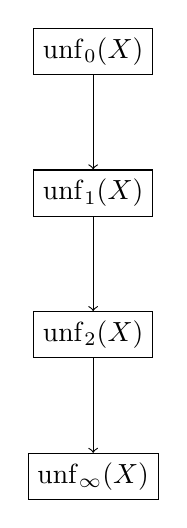
\begin{tikzpicture}[node distance=1.8cm]
    \node (x0) [rectangle, draw] {$\mathrm{unf}_0(X)$};
    \node (x1) [rectangle, draw, below of=x0] {$\mathrm{unf}_1(X)$};
    \node (x2) [rectangle, draw, below of=x1] {$\mathrm{unf}_2(X)$};
    \node (xinfty) [rectangle, draw, below of=x2] {$\mathrm{unf}_\infty(X)$};
    \draw[->] (x0) -- (x1);
    \draw[->] (x1) -- (x2);
    \draw[->] (x2) -- (xinfty);
  \end{tikzpicture}}

% Diagram C — Morphism of WARPs
\newcommand{\DiagramWARPmorphism}{
  \begin{tikzpicture}[>=stealth, node distance=2cm]
    \node[circle, draw] (Xv1) {$v_1$};
    \node[circle, draw, right of=Xv1] (Xv2) {$v_2$};
    \draw[->] (Xv1) -- (Xv2);
    \node[circle, draw, below=2cm of Xv1] (Yv1) {$v'_1$};
    \node[circle, draw, right of=Yv1] (Yv2) {$v'_2$};
    \draw[->] (Yv1) -- (Yv2);
    \draw[->, thick] (Xv1) -- (Yv1);
    \draw[->, thick] (Xv2) -- (Yv2);
  \end{tikzpicture}}

% Diagram D — Embedding ordinary graph
\newcommand{\DiagramGraphEmbedding}{
  \begin{tikzpicture}[>=stealth, node distance=2.2cm]
    \node[circle,draw,minimum size=0.7cm] (a) {$a$};
    \node[circle,draw,minimum size=0.7cm,right of=a] (b) {$b$};
    \draw[->] (a) -- node[above] {$e$} (b);
    \node[below=0.8cm of a] (aa) {\footnotesize $\Atom(p_\bullet)$};
    \node[below=0.8cm of b] (bb) {\footnotesize $\Atom(p_\bullet)$};
    \node at ($(a)!0.5!(b)+(0,-1.2)$) {\footnotesize $\Atom(p_\bullet)$ on $e$};
    \draw[dashed] (a) -- (aa);
    \draw[dashed] (b) -- (bb);
    \draw[dashed] ($(a)!0.5!(b)$) -- ($(a)!0.5!(b)+(0,-0.6)$);
  \end{tikzpicture}}
